% This is "sig-alternate.tex" V1.9 April 2009
% This file should be compiled with V2.4 of "sig-alternate.cls" April 2009
%
% This example file demonstrates the use of the 'sig-alternate.cls'
% V2.4 LaTeX2e document class file. It is for those submitting
% articles to ACM Conference Proceedings WHO DO NOT WISH TO
% STRICTLY ADHERE TO THE SIGS (PUBS-BOARD-ENDORSED) STYLE.
% The 'sig-alternate.cls' file will produce a similar-looking,
% albeit, 'tighter' paper resulting in, invariably, fewer pages.
%
% ----------------------------------------------------------------------------------------------------------------
% This .tex file (and associated .cls V2.4) produces:
%       1) The Permission Statement
%       2) The Conference (location) Info information
%       3) The Copyright Line with ACM data
%       4) NO page numbers
%
% as against the acm_proc_article-sp.cls file which
% DOES NOT produce 1) thru' 3) above.
%
% Using 'sig-alternate.cls' you have control, however, from within
% the source .tex file, over both the CopyrightYear
% (defaulted to 200X) and the ACM Copyright Data
% (defaulted to X-XXXXX-XX-X/XX/XX).
% e.g.
% \CopyrightYear{2007} will cause 2007 to appear in the copyright line.
% \crdata{0-12345-67-8/90/12} will cause 0-12345-67-8/90/12 to appear in the copyright line.
%
% ---------------------------------------------------------------------------------------------------------------
% This .tex source is an example which *does* use
% the .bib file (from which the .bbl file % is produced).
% REMEMBER HOWEVER: After having produced the .bbl file,
% and prior to final submission, you *NEED* to 'insert'
% your .bbl file into your source .tex file so as to provide
% ONE 'self-contained' source file.
%
% ================= IF YOU HAVE QUESTIONS =======================https://github.com/Boidkan/Senior_seminar_templates.git
% Questions regarding the SIGS styles, SIGS policies and
% procedures, Conferences etc. should be sent to
% Adrienne Griscti (griscti@acm.org)
%
% Technical questions _only_ to
% Gerald Murray (murray@hq.acm.org)
% ===============================================================
%
% For tracking purposes - this is V1.9 - April 2009

\documentclass{sig-alternate}
\usepackage{color}


%%%% User-defined macros
\newcommand{\lam}{\lambda}
\newcommand{\mycomment}[1]{\textcolor{red}{#1}}
%%%%% Uncomment this line (and comment the previous one)
%%%%% to remove all comments
%%%%% NOTE: comments still occupy a line even if invisible;
%%%%% Don't write them as a separate paragraph
%\newcommand{\mycomment}[3]{}

\begin{document}

%
% --- Author Metadata here ---
\conferenceinfo{UMM CSci Senior Seminar Conference, April 2014}{Morris, MN}
%\CopyrightYear{2007} % Allows default copyright year (200X) to be over-ridden - IF NEED BE.
%\crdata{0-12345-67-8/90/01}  % Allows default copyright data (0-89791-88-6/97/05) to be over-ridden - IF NEED BE.==
% --- End of Author Metadata ---

\title{Evolving Bytecode and Assembly}
%\subtitle{[Extended Abstract]
%
% You need the command \numberofauthors to handle the 'placement
% and alignment' of the authors beneath the title.
%
% For aesthetic reasons, we recommend 'three authors at a time'
% i.e. three 'name/affiliation blocks' be placed beneath the title.
%
% NOTE: You are NOT restricted in how many 'rows' of
% "name/affiliations" may appear. We just ask that you restrict
% the number of 'columns' to three.
%
% Because of the available 'opening page real-estate'
% we ask you to refrain from ElenaSampleputting more than six authors
% (two rows with three columns) beneath the article title.
% More than six makes the first-page appear very cluttered indeed.
%
% Use the \alignauthor commands to handle the names
% and affiliations for an 'aesthetic maximum' of six authors.
% Add names, affiliations, addresses for
% the seventh etc. author(s) as the argument for the
% \additionalauthors command.
% These 'additional authors' will be output/set for you
% without further effort on your part as the last section in
% the body of your article BEFORE References or any Appendices.
\numberofauthors{1} %  in this sample file, there are a *total*
% of EIGHT authors. SIX appear on the 'first-page' (for formatting
% reasons) and the remaining two appear in the \additionalauthors section.
%
\author{
% You can go ahead and credit any number of authors here,
% e.g. one 'row of three' or two rows (consisting of one row of three
% and a second row of one, two or three).
%
% The command \alignauthor (no curly braces needed) should
% precede each author name, affiliation/snail-mail address and
% e-mail address. Additionally, tag each line of
% affiliation/address with \affaddr, and tag the
% e-mail address with \email.
%
% 1st. author
\alignauthor
Eric C. Collom \\
\affaddr{University of Minnesota, Morris} \\
\email{coll0474@morris.umn.edu}
}

\maketitle
\begin{abstract}

\end{abstract}


\keywords{evolutionary computation, x86 assembly code, Java bytecode, FINCH, automated bug repair}

\section{Introduction}
Evolutionary Computation (EC) is a methodology, based off of evolutionary biology, that is used to solve problems. Similarly Genetic Programming (GP) is used to solve programs as the problem. However, traditional GP has been used mostly to solve only specific parts of problems, in programs, and not full-fledged programs themselves. Orlov et al.,~\cite{FINCH2:2009} purposes a method of applying GP to full-fledged programs. This method only requires a program to be able to be compiled to Java bytecode. Once in Java bytecode GP is applied to the program to solve the desired problem. Eric et al.,~\cite{Assembly:2010} also apply a similar method with bot Java bytecode and x86 assembly.\par
	Both Orlov et al.,~\cite{FINCH:2011} and Eric et al.,~\cite{Assembly:2010} show that this methodology is feasible by solving an array of problems. Orlov et al.,~\cite{FINCH2:2011} focused on automating solving simple programs while Eric et al., ~\cite{Assembly:2010} focused on automated bug repair in programs. 
	
Section 2 covers the background needed to understand this paper. It contains information on Evolutionary Computation (EC), x86 assembly, and Java bytecode. Section 3 covers the benefits of evolving assembly and bytcode. Section 4 discusses how Orlov, et al.,~\cite{FINCH:2011} evolve Java bytcode. We will cover similar work in section 5 by Eric, et al., on both x86 assembly and Java bytecode. In section 6 we will discuss the results from both Orlov et al.,~\cite{FINCH:2011} and Eric et al.,~\cite{Assembly:2010} experiments. In section 7 we will discuss future work that could be achieved with evolving 
	
	

\section{Background}
In this section we will explain what EC and GP, their components, and how they are used.
We will also discuss what x86 and Java bytecode is. Additionally we will also go over basic details of the JVM.
\subsection{Evolutionary Computation}

EC is a field of computer science and artificial intelligence that involves continuous optimization to solve problems. Optimization in EC is the selection of the best element within a set. Traditionally each element in a set is called an individual, and the set is called the population. A methodology used to apply continuous optimization, to solve programs as the problem, is GP. A GP evolves an initial population of programs either until the desired solution to the problem is found, or a specified number of generations is reached. To evolve an individual is to make changes to it. The fitness of each individual is the deciding factor on how likely it is chosen for evolution. The fitness is a value which indicates how well we think they solve the specific problem. For the research discussed in this paper a higher fitness indicates a more fit individual. One way that individuals are chosen to procreate is through tournament selection, where a certain number of individuals are chosen to compete and the individual with the highest fitness wins and then is selected for procreation. A way that procreating is implemented in GP is through the genetic operator called crossover. Crossover is the process of taking two individuals and extracting a section of code from one and replacing it with a section from the other program to form an offspring. Another genetic operator that is used to produce offspring is mutation. Mutation takes a program and then randomly changes a section of it. Mutation can be used along with crossover to produce offspring. Also, in some cases, the most fit individuals are passed on to the next generation unchanged, which is called elitism.


\subsection{x86 Assembly \& Java Bytecode}

\mycomment{need to explain stacks and frames}

Through out the rest of the paper I will use the term instruction-level code when referring to both Java bytecode and x86 assembly together. Instruction level code consist of operation codes (opcodes) which are each one byte in length. Hover, some opcodes that take parameters are multiple bytes long~\cite{JavaBytecode:2014,x86tomachine:2013}.

\subsubsection{X86}
x86 is a family of backward compatible low-level programming languages~\cite{x86:2014} created by Intel and designed for specific computer architectures. This means that it is designed to only run on certain physical machines. This is one of the main differences between x86 assembly and Java bytcode. 

\subsubsection{ Bytcode And The JVM}
Java bytecode ``is the intermediate, platform-independent representation''~\cite{VIII:2011} originaly designed for the Java compiler. However, other high-level languages now also have compilers for the Java Virtual Machine (JVM). Some of those languages are Scala, Groovy, Jython, Kawa, JavaFx Script, Clojure~\cite{FINCH:2011}, Erjang, and JRuby. 

The JVM executes bytecode through a stack-based architecture. Each JVM thread has a private stack, and each stack stores frames. Each frame contains an array of local variables, its own operand stack, and a reference to the class of the current method. Only the frame of the current executing method can be active at a time.


\subsection{Grammar Stuff}

\paragraph{Backus-Naur Form}
	Backus-Naur Form(BNF)~\cite{BNF:2014} is a notation technique used for context free grammars (CFG) and is used to represent the syntax of computer programming languages.





\section{The Benefits}

There are many problems we run into when trying to evolve source code. One problem is that it is extremely difficult to evolve an entire program due to source code syntactical constraints. Another problem is that we cannot just take a program and evolve it, we have to design  a GP for that specific problem. Evolving instruction-level code bypasses both of these problems.

\begin{figure}
\centering
{\tt
\begin{verbatim}
float x;                    int x=7;
int y=7;                    float y;
if(y>=0){                   if(y>=0){
    x=y;                        y=x;
}else{                          x=y;
    x=-y;                   }
}System.out.println(x);      System.out.println(z);	
     
     (a)                      (b)

\end{verbatim}
}
\caption{Both (a) and (b) are valid code syntactically however only (a) is valid semanticly.}
\end{figure}


\begin{figure}
\centering
{\tt
\begin{verbatim}
class SymbolicRegression{
    Number symbolicRegression(Number num){
        double x = num.doubleValue();
        return Double.valueOf((x+x)*x);
    }
}
\end{verbatim}
}
\caption{Example of a possible starting program to evolve and solve symbolic regression.}
\end{figure}

\begin{figure}
\centering
{\tt
\begin{verbatim}
Bytcode    Frame1  

iload_1	   class	
iload_2    1
iadd       3
ireturn


Execute iload_1  Execute iload_2   

    Stack            Stack            
      1                1               
                       3
                       
Execute iadd     Execute ireturn

  Stack           Stack(empty)
    4


          
\end{verbatim}
}
\caption{Istore\_n pushes an element from index n from frame onto stack. Iadd pops two elements from operand stack add them together and then pushes to the result to the stack. Ireturn pops an element from the stack and returns it}
\end{figure}

%\begin{figure}
%\centering
%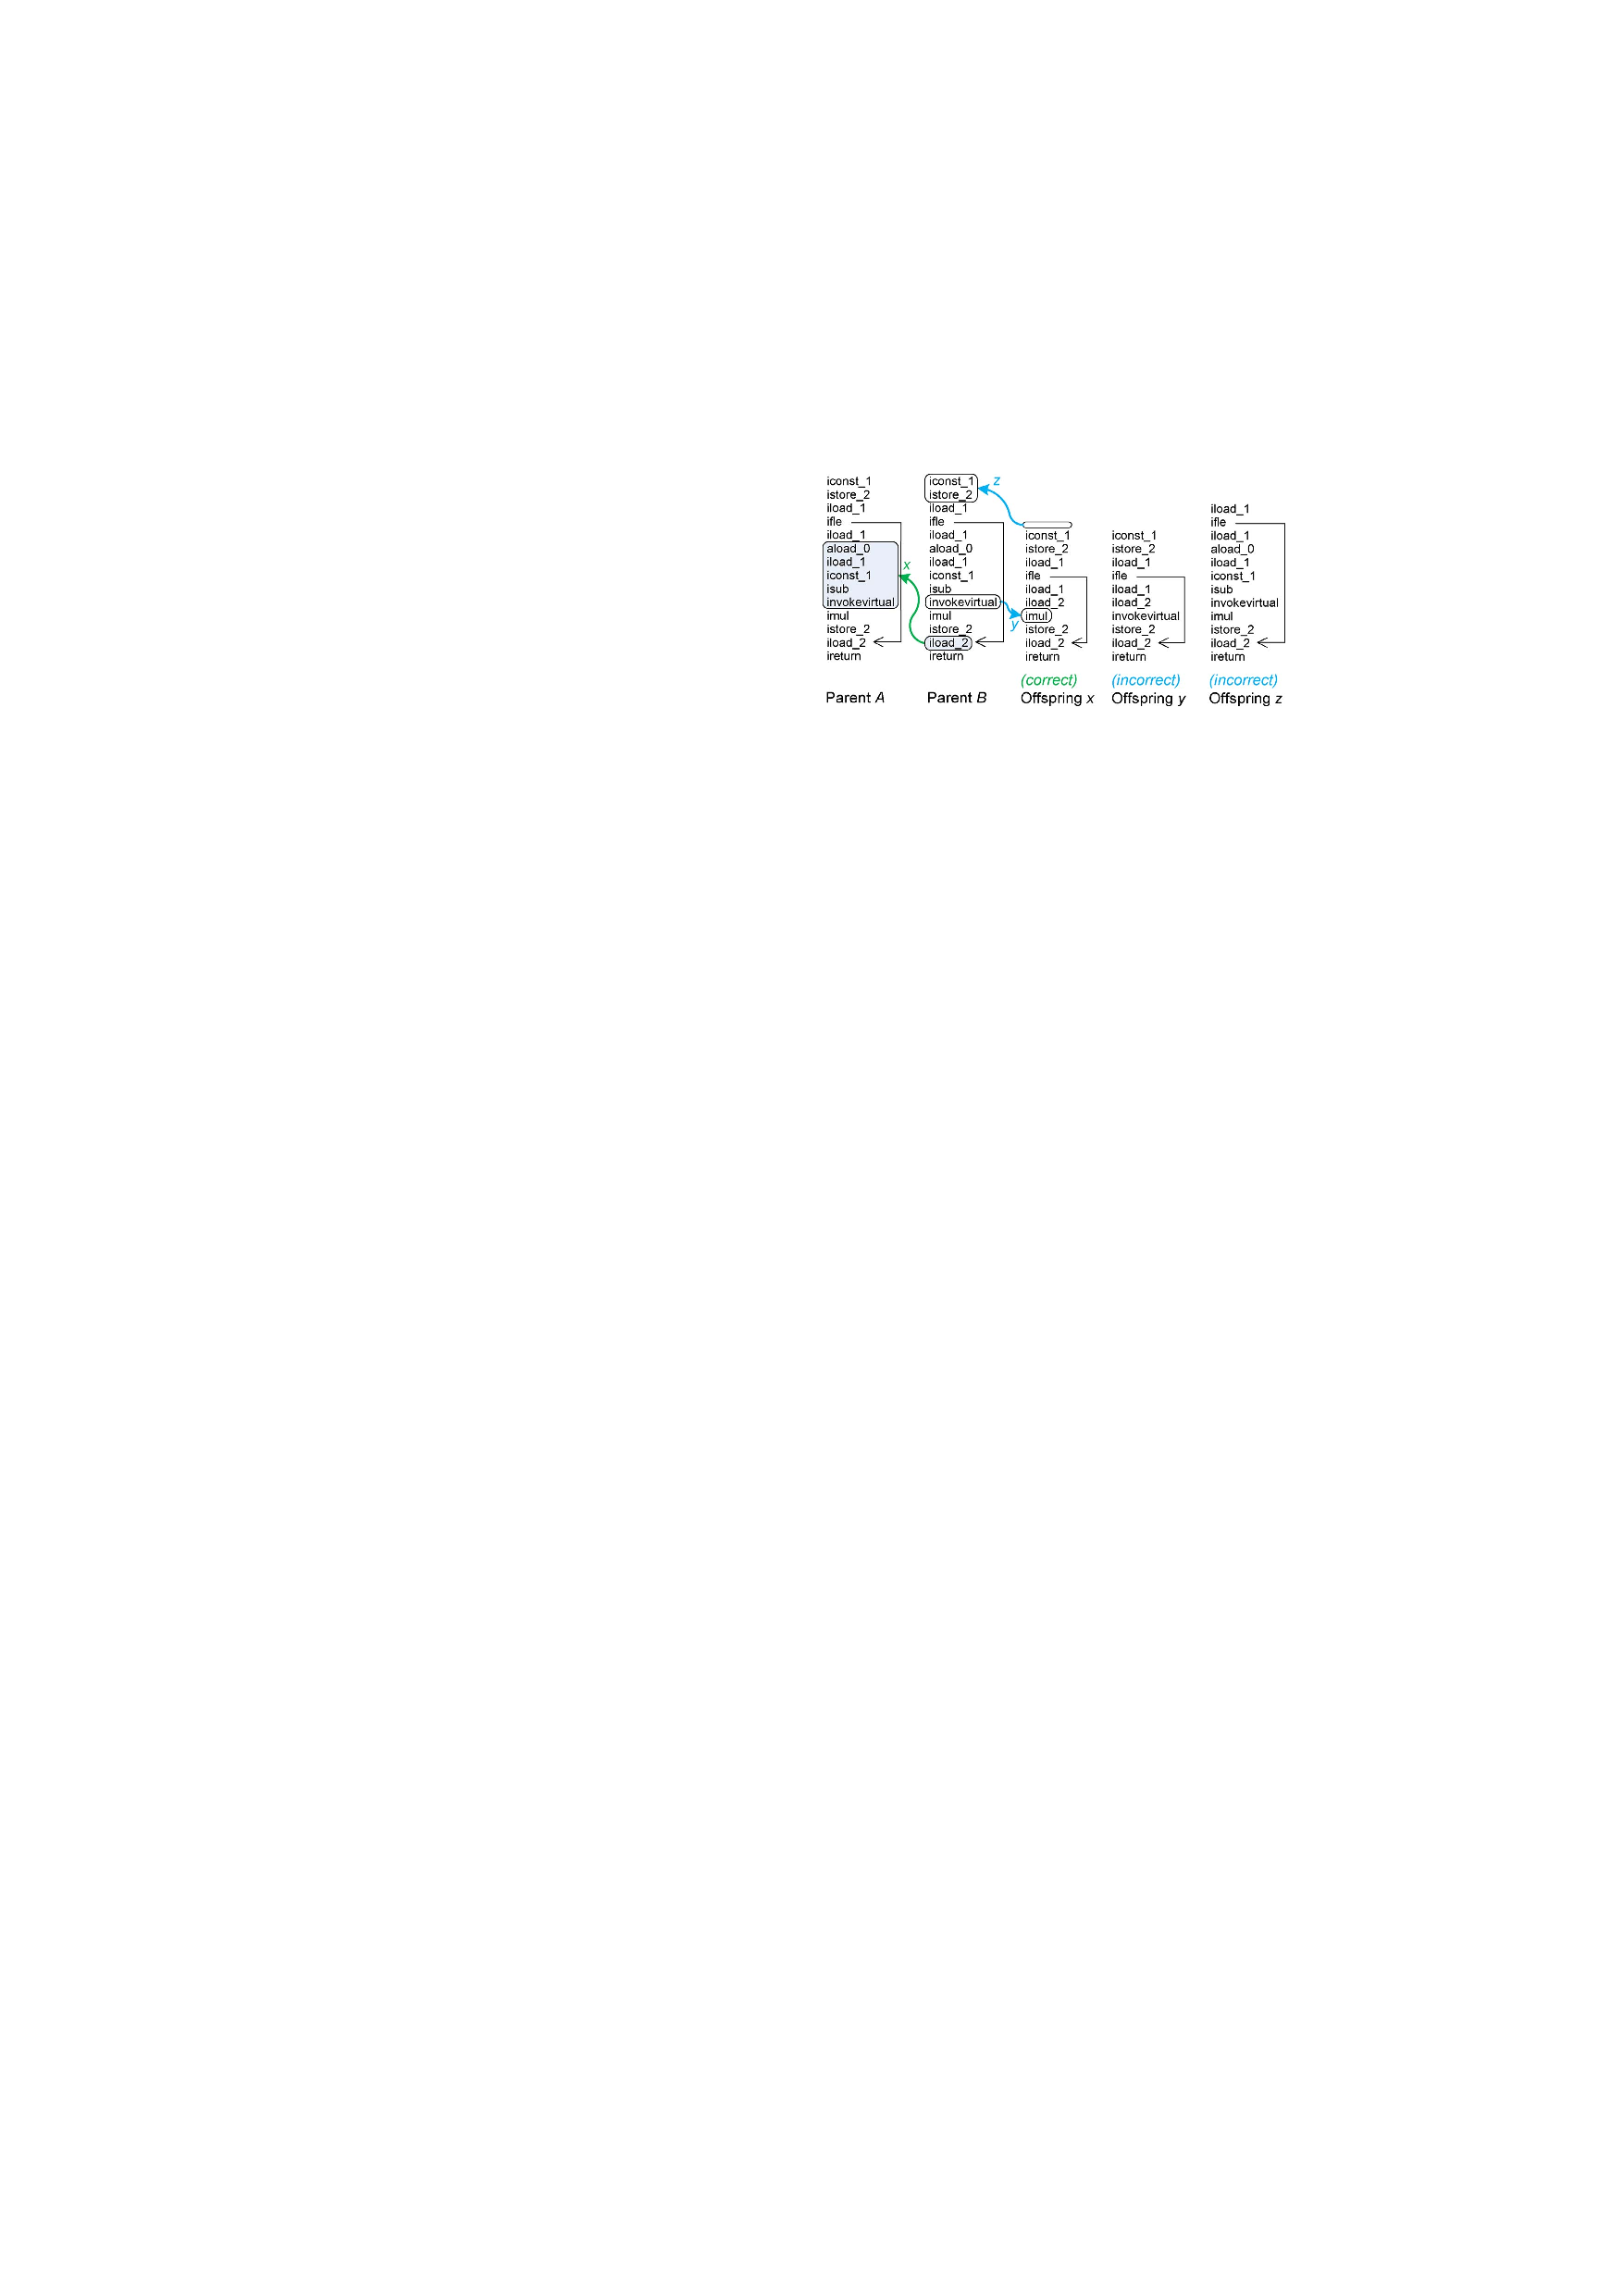
\psfig{file=bytecode.pdf}
%\caption{Java Bytcode}
%\end{figure}



\subsection{Source Code Constraints}
One problem with trying to evolve entire programs at the source code level is that there is a very high risk of producing a non-compilable program. This is due to the fact that high-level programming languages are designed to make it easy for humans to read and write programs. Most high-level programming languages are defined using grammars which are used to represent the syntax of the programming language~\cite{Oracle:2013,Assembly:2010}. This means that the grammar does not represent the semantic constraints of a program. The grammar does not capture the languages type system, variable visibility and accessibility, and other constraints ~\cite{FINCH:2011}. For example, in figure 1 both 1.(a) and 1.(b) comply to the syntactical rules of Java. However, when taking into account semantics 1.(b) is illegal code. In 1.(b) variable \texttt{y} is uninitialized before the test in the if statement, and assigning \texttt{y} to \texttt{x} violates a type constraint. Plus, variable \texttt{z} is not defined anywhere.  In order to write a program to evolve source code we would have to deal with all these constraints. While this task is possible it would require creating a full-scale compiler to check for these semantic constraints. Thus, it is easier to evolve instruction-level code. \par

Instruction-level code consist of a small set of instructions~\cite{Assembly:2010}. They are simpler syntactically and there are less semantic constraints to violate. This means that there is a lower risk of producing a noncompilable program during evolution. 

\subsection{Evolving As Is}
In tradition EC when creating a GP to evolve a program there is a lot of scaffolding that has to be done. Usually we have to design the GP for that specific program. When a GP is designed it is common to just evolve expressions or formulae ~\cite{FINCH:2011} within the program. Most of the program as a whole would be already written and remain the same after evolution. The GP has to know what it can evolve and where it is located. Also, usually the GP isn't useful in evolving other programs to contain different problems. Instead an entirely new GP would have to be designed and the program along with it.

When evolving instruction-level code there is no requirement for the program being evolved to be designed for the GP. The GP doesn't have to focus on a specific part of the program or even be aware of what is in the program for the most part. Instead the program that is being evolved stays as is and the GP goes through minor modifications to fit the problem trying to be solved. The GP has to be given a fitness algorithm in order to attempt to find a desirable individual. It also needs to know what genetic operator and the desired number of generations is needed. Depending on the on the program being evolved one might also have to put a growth limit on the code or implement protected division or logarithm. For example, Orlov et al.,~\cite{FINCH:2011} enforced a growth limit when performing crossover on code so that the programs would not become too large. The initial population can also almost contain no code in it in order for the GP to find a desirable solution. 

A huge benefit that comes from most of the scaffolding happening on GP end is that the initial program being evolved does not have to contain a whole lot of code. The GP can evolve a minimal amount of code into a full-scale working program. However, evolving instruction-level code is also capable of being very focused like traditional GP is on source code. For example, Eric et al.,~\cite{Assembly:2010} in their research focused on only evolving small areas of code and would only make minor changes to the code as a whole. The result code would usually only have one line of code changed. 




\section{FINCH}
FINCH is a program developed by Orlov et al.,~\cite{FINCH2:2009,FINCH:2011} that evolves programs that have already been compiled into Java bytecode.

\subsection{Crossover}

\begin{figure}
\centering
{\tt
\begin{verbatim}
1.   iconst_1    iconst_4    iconst_4    iconst_4
2.   iconst_3    iconst_2    iconst_2    istore_1
3    istore_1    istore_1    istore_1    istore_2
4    istore_2    istore_2    istore_2    istore_2
5.   iload_1     iload_1     iload_2     iload_2
6.   iload_2     iload_2     iload_2     iload_1
7.   iadd        isub        isub        isub
8.   ireturn     ireturn     ireturn     ireturn
9.                          
      (A)          (B)         (C)          (D)
          
\end{verbatim}
}
\caption{Iconst\_n pushes an int n onto the stack. Istore pops the stack and saves the element on the frame. storesIstore\_n pushes an element from index n from frame onto stack. Iadd pops two elements from operand stack add them together and then pushes to the result to the stack. Ireturn pops an element from the stack and returns it}
\end{figure}


The FINCH uses two-point crossover to evolve Java bytecode. It takes two programs A and B and extracts sections $\alpha$ and $\beta$ respectively. It then takes section $\alpha$ and inserts it into where section $\beta$ used to be. It only selects an $\alpha$ that will compile after being inserted into B. Take into account that just because $\alpha$ can replace $\beta$ in B does not imply that $\beta$ can replace $\alpha$ in A. In other words it is not a biconditional relationship.

For example in Figure 4 let the Java bytecode snippets 4(A) and 4(B) be A and B. Let $\alpha$ be line 6 from A and $\beta$ be line 5 from B. A(C) is the product of replacing $\beta$ with $\alpha$ in B. A(C) is good crossover. Now let $\alpha$ be lines 3-4 in A and $\beta$ be lines 2-3 in B. A(D) is the result of replacing $\beta$ with $\alpha$ in B. However in this case A(D) is incorrect crossover since only one integer is saved on the frame and at line 3 istore\_2 tries to pop an empty stack causing stack underflow.


\subsection{Selecting Offspring}
Evolving Java Byte code only reduces the chance of evolving non-compilable bytecode to a certain extent. Even though Java byte code has a simpler syntax than source code, it still has syntactical constraints. Orlov et al.,\cite{FINCH2:2009} address this issue by checking if a good offspring has been created before letting it join the evolved population, thus ensuring offspring produced through crossover contain valid bytcode. If an illegal offspring is produced then another offspring with the same parents is made. This process is repeated until a good offspring is produced or a predetermined number of attempts have been made.\par
These checks makes sure that stack depth, variable type, and control flow is respected.

\paragraph{Stack and Variable Types}
The following checks are done to assure that the stack and stackframe are both type compatible and stack underflow does not happen. Stack underflow is where an attempt to pop from an empty stack occurs. Stack pops of $\beta$ must have identical or narrower types and depth as $\alpha$. Stack pushes of $\alpha$ must have identical or narrower types as stack pushes of $\beta$.

\paragraph{Variable Types}
The following checks are done within the bytcode to make sure that by inserting $\alpha$ into $\beta$ that variables written before and after those sections are compatible with the change. 
First, variables written by $\alpha$ must have identical or narrower types that are read after $\beta$. It is also made sure that all variables read after $\beta$ and not written by $\alpha$ must be written before $\beta$.Finally, all variables read by $\alpha$ must be written before $\beta$.

\paragraph{Control flow}
These checks are done to make sure that when jumps within the bytcode is done that it doesn't cause the program to break. First, a check is done to make sure that there are no jumps in $\beta$ and jumps out of $\alpha$. Secondly, a check is done to make sure that the code before $\beta$ transitions into $\beta$ and that $\alpha$ transitions into code post $\alpha$.  


The checks make sure that all the variables will be read, written, type-compatible, and will not cause stack underflow\cite{VIII:2011}. For example, in figure 1, if 1.(b) was the result of two parent programs then it would be rejected as a good offspring due to its failure to comply to semantical constraints stated Section 3.1.\par
It is important that only good offspring is selected because this provides good variability in the population. Good variability is where there are many that vary in code and fitness. Noncompilable code would result in a fitness score of zero. Since noncompilable code would occur frequently enough it would cause a large portion of the population to have a zero fitness score. This would possibly result in having individuals with a zero fitness being selected for procreation and thus consistently resulting in bad crossover and bad offspring.


Orlov et al.~\cite{FINCH:2011} focused on evolving small programs to solve problems. The five problems they focused on were symbolic regression, artificial ant, intertwined spirals, array sum, and tic-tac-toe. We will discuss their results from the symbolic regression and array sum problems. Their program, FINCH, was able to evolve programs and solve each of these problems.

In each of tests FINCH was given each time a program that had a zero fitness. The elements included in the programs were the minimal components to successfully evolve and solve the problem. For example, in the case of symbolic regression the initial population contained the mathematical function set \{+, -, *, \%, $sin$, $cos$, $e$,  $ln$\} and number types.

\subsection{Non-Halting Offspring}
Another issue that arises from evolving unrestricted bytcode is that the resulting program might enter a non-halting state. These problems do not arise when the check to see if an offspring is good bytecode. Instead, this is a runtime issue. This, is especially true when evolving programs that contain loops and recursion.
The way that Orlov et al.,~\cite{FINCH:2011} deal with this, before running the program, is count how many calls are made to each function. If too many calls are made to a function than an exception is thrown. They do not specify what fitness is assigned to an individual that fails this test.






\section{Evolving Assembly Code}
Eric, et al, focus evolving x86 and Java Bytecode for the purpose of program repair and debugging. In their tests they took medium to large sized programs in Java, C, and Haskell that contained a bug. The types of bugs they used were common human errors such as having a for loop index off by one. Most of their experiments focused on evolving a small section of the program.
\subsection{Fitness and Selecting Good Offspring } 
In selecting offspring a different path was chosen than Olov, et al. They decided to not make sure produced offspring were compilable. Instead they decided to let all produced offspring into the next generation. This produced a considerable amount of individuals with fitness zero due to being noncompilable. 

Each program to be evolved was provided with a set of tests that passed and one test that failed. The failed test was used to check if an offspring fixed the bug. The tests that passed were used to make sure the program retained functionality. For each offspring they compiled them into either an executable binary(x86) or class file (Java). If the program failed to compile then it would obtain a fitness of zero. If the program did compile then it was ran with the tests. The fitness score is calculated as the weighted sum of tests passed, the negative test being worth more. This a great weight was placed on the non passing testing since that was the main goal.

  

\subsection{Genetic Operators}
Eric, et al., used mutation on 90\% of each population and crossover on the rest to produce the offspring population. Multiple tournaments consisting of three individuals were performed to select fit individuals for reproduction. They used mutation over crossover 90\% of the time because it produced better results for the type of problems they were solving. Since, each bug was a minor change, such as change a zero to a one, using a large amount of crossover or more complex operators generally slowed their search time.  

\subsection{Non-Halting Offspring}

Eric, et al., also chose a different approach than that of Olav, et al., when dealing with non-halting offspring. They decided to not check for non-halting and instead run the individual on a virtual machine(VM) with an eight second timeout on the process. Olov, et al., decided against this due to two main issues. First it is hard to define how long a program should run which can vary greatly depending on the cpu load. Thus if good time limit is not selected then it can be waste to cpu resources. The second issue is that limiting the runtime requires running the program on a separate thread. Killing the thread can be unreliable and can be unsafe for the GP as a whole. Eric, et al., ran into the problem where sometimes programs would not respond to termination requests.
They also ran into "Stack Smashing" which is where the stack of the application or operator overflow which can cause the program and system as a whole to crash. However, since they ran each individual on a VM stack smashing was not a significant problem.




\section{Results}
\subsection{FINCH}
Orlov et al.~\cite{FINCH:2011} focused on evolving small programs to solve problems. The five problems they focused on were symbolic regression, artificial ant, intertwined spirals, array sum, and tic-tac-toe. We will discuss their results from the symbolic regression and array sum problems. Their program, FINCH, was able to evolve programs and solve each of these problems.

In each of tests FINCH was given each time a program that had a zero fitness. The elements included in the programs were the minimal components to successfully evolve and solve the problem. For example, in the case of symbolic regression the initial population contained the mathematical function set \{+, -, *, \%, $sin$, $cos$, $e$,  $ln$\} and number types.


\subsubsection{Symbolic Regression}
Symbolic regression is a method of finding a mathematical function that best fits a a set of points between two intervals. Olov, et al.,~\cite{FINCH:2011} chose to use 20 random points, between -1 and 1, from various polynomials. Fitness was calculated as the number of points hit by the function. The function set \{+, -, *, \%, sin, cos, $e$, $ln$\}(note: referring to $e$ as a function in the Java.lang.Math library) was used for most of their experiments. This was done in order to mimic previous experimentation done~\cite{koza:1992} in order to compare the results to traditional GP. They were able to evolve up to a 9-degree polynomial with just the function set \{+, *\}.

A more complex fitness was also tested. This symbolic regression consisted of a fitness that checked if all twenty points were within $10^{-8}$ degree of they polynomials output. 

For each experiment they started off with an offspring of fitness zero and usually with a minimal amount of code, such as in figure 2. They evolved the programs with a 90\% crossover. Using the simple fitness algorithm 99\% of the time a maximum fitness individual was found. With the more complex fitness algorithm a maximum fitness individual was found 100\% of the time.


\subsubsection{Array Sum}
The array sum problem consists of adding up all the values in an array. This problem is important because it would require evolving a loop or recursion to solve it. This would show that FINCH is capable of evolveing more complex programs\par
FINCH was able to solve this problem quite easily though recursion and a for loop. This experiment also showed that FINCH is able to evolve different list abstractions such as List and ArrayList.\mycomment{this section in the papscannerer is short. Should I include some their code to show their results and as an example?} 


\subsection{x86}
\mycomment{looking into other research/papers by this group to get more to write about.}

Eric,et al., were able to show that it is possible to fix human programming errors though bytecode and assembly. They were able to successfully debug various programs containing bugs such as infinite loops and remote buffer overflows.

Even though they produced a considerable amount of offspring with fitness zero this did not seem to hurt their result very much. The average number of fitness evaluations required to produce an offspring that passed all the tests was 63.6 for C and 74.4 for assembly. This indicates that not much more work is needed to to evolve repairs in assembly. Even programs that contained thousands of lines of code only required a few runs. This shows that evolving programs in assembly is feasible. \mycomment{include weighted path?}

It was also discovered that most repairs only required a small number of operations. This was also due to optimization of mutation.\mycomment{not much info is provided on this}


\subsection{Future Work}



\section{Conclusion}

%\end{document}  % This is where a 'short' article might terminate

%ACKNOWLEDGMENTS are optional
\section{Acknowledgments}


%
% The following two commands are all you need in the
% initial runs of your .tex file to
% produce the bibliography for the citations in your paper.
\bibliographystyle{abbrv}
\bibliography{EricBibliography}  % ElenaSample.bib is the name of the Bibliography in this case
% You must have a proper ".bib" file
%  and remember to run:
% latex bibtex latex latex
% to resolve all references
%
% ACM needs 'a single self-contained file'!
%
%APPENDICES are optional
%\balancecolumns

\end{document}

\appendix
%Appendix A
\section{Headings in Appendices}
The rules about hierarchical headings discussed above for
the body of the article are different in the appendices.
In the \textbf{appendix} environment, the command
\textbf{section} is used to
indicate the start of each Appendix, with alphabetic order
designation (i.e. the first is A, the second B, etc.) and
a title (if you include one).  So, if you need
hierarchical structure
\textit{within} an Appendix, start with \textbf{subsection} as the
highest level. Here is an outline of the body of this
document in Appendix-appropriate form:
\subsection{Introduction}
\subsection{The Body of the Paper}
\subsubsection{Type Changes and  Special Characters}
\subsubsection{Math Equations}
\paragraph{Inline (In-text) Equations}
\paragraph{Display Equations}
\subsubsection{Citations}
\subsubsection{Tables}
\subsubsection{Figures}
\subsubsection{Theorem-like Constructs}
\subsubsection*{A Caveat for the \TeX\ Expert}
\subsection{Conclusions}
\subsection{Acknowledgments}
\subsection{Additional Authors}
This section is inserted by \LaTeX; you do not insert it.
You just add the names and information in the
\texttt{{\char'134}additionalauthors} command at the start
of the document.
\subsection{References}
Generated by bibtex from your ~.bib file.  Run latex,
then bibtex, then latex twice (to resolve references)
to create the ~.bbl file.  Insert that ~.bbl file into
the .tex source file and comment out
the command \texttt{{\char'134}thebibliography}.
% This next section command marks the start of
% Appendix B, and does not continue the present hierarchy
\section{More Help for the Hardy}
The sig-alternate.cls file itself is chock-full of succinct
and helpful comments.  If you consider yourself a moderately
experienced to expert user of \LaTeX, you may find reading
it useful but please remember not to change it.
%\balancecolumns % GM June 2007
% That's all folks!
\end{document}
